%\documentclass[12pt]{article}
\documentclass[10pt,fleqn,twoside]{article}

\usepackage{epsfig}
\usepackage{float}
\usepackage{color}

%%%% USE ARIAL FONT %%%%%%%%%%%%%%%%%%%%%%%%%%%%%%%%%%%%%%%%%%%%%%%%%%%%%%
\usepackage{helvet}
\renewcommand\familydefault{phv}

%%%% INCLUDE NECESSARY PACKAGES %%%%%%%%%%%%%%%%%%%%%%%%%%%%%%%%%%%%%%%%%%
%\usepackage{babel}
\usepackage[UKenglish]{babel}
\usepackage{amsmath}
\usepackage{amssymb}
\usepackage{fancyhdr}
\usepackage{natbib}
\usepackage{ae,aecompl}
\usepackage{graphicx}
\usepackage{palatino}
\usepackage[T1]{fontenc}
\usepackage[right]{eurosym}
\usepackage{rotating}
\usepackage{epsf}
\usepackage{setspace}
\usepackage{xspace}
\usepackage{multicol}
\usepackage{siunitx}
%\usepackage{caption}

\usepackage{sfmath}

\usepackage[utf8]{inputenc}

% ========= hyperref & Colors & Links ===========
\usepackage[usenames,dvipsnames]{xcolor}
%\usepackage[breaklinks]{hyperref}
\usepackage{hyperref}
\addto\extrasUKenglish{%
\def\sectionautorefname{Section}%
\def\subsectionautorefname{Section}%
\def\subsubsectionautorefname{Section}%
\def\paragraphautorefname{Section}%
}
\usepackage[all]{hypcap} % fixes links to floats
\usepackage{aas_macros}  %
\setlength{\bibsep}{-0.5pt}

% ========= highlighting important parts of the proposal ===========
\definecolor{HighLight}{rgb}{0.9,0.3,0.0}
%\newenvironment{highlight}{\color{blue}\itshape}{\ignorespacesafterend}
%\newenvironment{highlight}{\color{RedOrange}\itshape}{\ignorespacesafterend}
%\newenvironment{highlight}{\color{RedOrange}\bfseries}{\ignorespacesafterend}
%\newenvironment{highlight}{\color{BrickRed}\bfseries\itshape}{\ignorespacesafterend}
%\newenvironment{highlight}{\color{BrickRed}\bfseries}{\ignorespacesafterend}
%\newenvironment{highlight}{\color{HighLight}\bfseries}{\ignorespacesafterend}
\newenvironment{highlight}{\color{HighLight}}{\ignorespacesafterend}
\newenvironment{missingenv}{\color{red}}{\ignorespacesafterend}

\definecolor{Emphasize}{rgb}{0.0,0.5,0.0}
\newenvironment{Emphasize}{\color{Emphasize}\itshape}{\ignorespacesafterend}


% strike through comments: to turn them off, uncomment the renewcommands below
\usepackage{soul}
\setstcolor{red}

% ========= Commands specially for the forschergruppe =========

\newcommand{\todo}[1]{\textcolor{red}{\bf #1}}
\newcommand\connect[1]{{\color{OliveGreen} #1}}

%%%% CAPTION LAYOUT %%%%%%%%%%%%%%%%%%%%%%%%%%%%%%%%%%%%%%%%%%%%%%%%%%%%%

\usepackage[font={small}]{caption}

%%%% PAGE LAYOUT %%%%%%%%%%%%%%%%%%%%%%%%%%%%%%%%%%%%%%%%%%%%%%%%%%%%%%%%%
\setlength{\textheight}{22cm}
\setlength{\topmargin}{-1.2cm}
\setlength{\textwidth}{15.6cm}
\setlength{\oddsidemargin}{0.0cm}
\setlength{\evensidemargin}{0.0cm}
\setlength{\mathindent}{1.5cm}
\setlength{\parindent}{0.0cm}
\setlength{\parskip}{0.08cm}

%%%% PAGE HEADER %%%%%%%%%%%%%%%%%%%%%%%%%%%%%%%%%%%%%%%%%%%%%%%%%%%%%%%%%%
\pagestyle{fancy}
\fancyhead[RE,RO]{}
\fancyfoot[RO]{\thepage}
\fancyfoot[LE]{\thepage}
\fancyfoot[CE,CO]{}

%%% FONTS FOR THE TITLE PAGE %%%%%%%%%%%%%%%%%%%%%%%%%%%%%%%%%%%%%%%%%%%%%%
\newfont{\tpfonta}{cmssbx10 scaled 1600}
\newfont{\tpfontb}{cmssbx10 scaled 3200}

%%%% COLOR DEFINITIONS %%%%%%%%%%%%%%%%%%%%%%%%%%%%%%%%%%%%
\definecolor{blue} {rgb} {0.25,0.25,0.75}

%%%% ADDITONAL EMPHASIS %%%%%%%%%%%%%%%%%%%%%%%%%%%%%%%%%%%
\newcommand{\cem}{\color{blue}}
\newcommand{\eem}{\sl\color{blue}}

%%%% BIBTEX PUNCTUATION %%%%%%%%%%%%%%%%%%%
\bibpunct{(}{)}{;}{a}{}{,} % to follow the A&A style

%%%% SET THE COLOR OF THE (SUB-) SECTION TITLES %%%%%%%%%%% 
\newcommand{\Tcol}{\color{blue}}

%%%% SET THE COLOR OF THE TITLE BOX BACKGROUND %%%%%%%%%%%%
\definecolor{Background}{rgb} {0.62,0.75,0.5}

%%%%%%%%%%%%%% REFERENCE SECTION NAME %%%%%%%%%%%%%%%%%%%%
\renewcommand\refname{\Tcol 9. Bibliography}

%%%%%%%%%%%%%% NICER PROJECT REFERENCES %%%%%%%%%%%%%%%%%%%

\newenvironment{literature}%
 {\begin{multicols}{2}\begin{scriptsize}\begin{list}{}{%
   \setlength{\topsep}{0em}%
   \setlength{\parskip}{0em}%
   \setlength{\parsep}{0em}%
   \setlength{\itemsep}{0em}%
   \setlength{\rightmargin}{0em}%
   \setlength{\leftmargin}{2em}%
   \setlength{\itemindent}{-2em}}}%
 {\end{list}\end{scriptsize}\end{multicols}}

%
% ...A compact itemize environment
%
\newenvironment{compactitemize}%
 {\begin{list}{$\bullet$}{%
   \setlength{\topsep}{0em}%
   \setlength{\parskip}{0em}%
   \setlength{\parsep}{0em}%
   \setlength{\itemsep}{0.0\baselineskip}%
   \setlength{\rightmargin}{0em}%
   \setlength{\leftmargin}{2.0em}%
   \setlength{\labelsep}{0.5em}%
   \setlength{\labelwidth}{1em}%
}}
 {\end{list}}

\newcounter{qcounter}
\newenvironment{compactenumerate}%
 {\begin{list}{\arabic{qcounter})~}{\usecounter{qcounter}%
   \setlength{\topsep}{0em}%
   \setlength{\parskip}{0em}%
   \setlength{\parsep}{0em}%
   \setlength{\itemsep}{0.0\baselineskip}%
   \setlength{\rightmargin}{0em}%
   \setlength{\leftmargin}{2.0em}%
   \setlength{\labelsep}{0.5em}%
   \setlength{\labelwidth}{1em}%
}}
 {\end{list}}

%%%% EXPLANATION FOR THE CONNECT COLOR %%%%%%%%%%% 
\newcommand{\footexplainconnect}{\footnote{The text highlighted in \connect{green} refers to the connection of this project to other projects of this Research Unit.}}
 
%%%%%%%%%%%%%%%%%% NICER REFERENCES %%%%%%%%%%%%%%%%%%%

%\usepackage[capitalise,nameinlink]{cleveref}
\newcommand{\cref}[1]{\autoref{#1}}

%%%%%%%%%%%%%%%%%% COLOR THE SECTION NUMBERS %%%%%%%%%%%%%%%%%

\makeatletter
\renewcommand\@seccntformat[1]{\color{blue} {\csname the#1\endcsname}\hspace{0.5em}}
\makeatother
\renewcommand\thesection{\arabic{section}.}
\renewcommand\thesubsection{\arabic{section}.\arabic{subsection}}

%%%%% color sections
\usepackage{sectsty}
\allsectionsfont{\color{blue}}


%%%% CHANGE THE APPEARANCE OF THE \PARAGRAPH COMMAND  %%%%%%%%%%%%%%%%%%%%%%%%%%%%%%%
\makeatletter
\renewcommand\paragraph{\@startsection{paragraph}{4}{\z@}%
            {-2.5ex\@plus -1ex \@minus -.25ex}%
            {1.25ex \@plus .25ex}%
            {\normalfont\normalsize\bfseries\Tcol}}
\makeatother
\setcounter{secnumdepth}{4}     % how many sectioning levels to assign numbers to
\setcounter{tocdepth}{4}        % how many sectioning levels to show in ToC

%%%%% set header

\renewcommand{\sectionmark}[1]{\markright{\color{black}#1}}

\newcommand{\caphighlight}[1]{{\bf #1}}



\def\team#1{{#1\/}}
\def\coll#1{{#1\/}}
%\def\remark#1{{\bf [#1]}}
\def\remark#1{}
\newcommand{\Titlecol}{\color{Black}}
\newcommand{\AreacolA}{\color{blue}}
\newcommand{\AreacolB}{\color{Green}}
\newcommand{\AreacolC}{\color{YellowOrange}}
\newcommand{\AreacolD}{\color{Red}}

\begin{document}

\pagestyle{empty}
\mbox{}
\vspace{1cm}\\

\centerline{\Titlecol\huge \bf Planet Formation Witnesses and Probes:}
\vspace{0.5cm}
\centerline{\Titlecol\huge \bf Transition Discs}
\vspace{2cm}
\centerline{\Titlecol\Large \bf Proposal for funding a DFG Research Unit}
\vspace{2cm}
\centerline{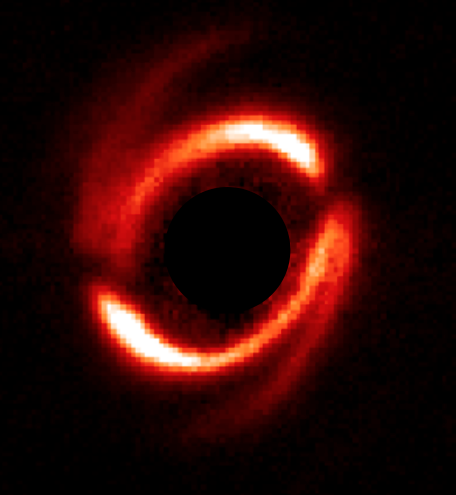
\includegraphics[width=0.6\textwidth]{figures/HD100453.png}}
\vspace{1cm}
\centerline{\Large Speaker: Barbara~Ercolano}
\vspace{0.5cm}
\centerline{\Large Co-speaker: Cornelis Dullemond}


\pagebreak[4]

\mbox{}
\vfill
Cover image: The Transition Disk HD 100453 as seen with the VLT-SPHERE 
instrument in scattered polarized light. From: Benisty et al.~2017,
A\&A in press.

\todo{NOTE: We have to ask permission from the main author (Myriam
Benisty) and the SPHERE consortium to use this image. We can also
use another image, or use a theoretical model.}

\pagebreak[4]


\section{Participating institutes and 
principle investigators
}\label{app-institutes}
\begin{itemize}
\item {\bf Ludwig Maximilians University Munich (LMU):}
 \begin{itemize}
  \item University Observatory\\    
         {\em (Prof.~Dr.~Barbara~Ercolano, Prof.~Dr.~Thomas~Preibisch,
           Dr.~Tilman Birnstiel)}
  \end{itemize} 
\item {\bf European Southern Observatory, Garching:}
 \begin{itemize} 
\item Star and planet formation group \\
         {\em (Dr.~Leonardo~Testi)}
\end{itemize}
\item {\bf Max-Planck-Institute for Extraterrestrial Physics, Garching:}
 \begin{itemize} 
\item Centre for Astrochemical Studies \\
         {\em (Prof.~Dr.~Paola~Caselli)}
\end{itemize}
\item {\bf Ruprecht-Karls-University Heidelberg:}
\begin{itemize}
 \item Institute for Theoretical Astrophysics (ITA)\\
         {\em (Prof.~Dr.~Cornelis~P.~Dullemond)}
\end{itemize}
\item {\bf University of T\"ubingen:}
\begin{itemize}
  \item Institute for Astronomy \& Astrophysics\\
         {\em (Prof.~Dr.~Wilhelm~Kley)}
\end{itemize}
\end{itemize}
%
\vfill

\noindent {\bf Speaker:}\\
Prof.~Dr.~Barbara~Ercolano \hfill Tel.: 089-2180-6974\\
University Observatory  \\
Ludwig Maximilians University Munich \hfill e-mail ercolano@usm.lmu.de\\
Scheinerstr 1, D-81679 M\"unchen\\

\noindent {\bf Co-speaker:}\\
Prof.~Dr.~Cornelis~P.~Dullemond \hfill Tel.: 06221-544815\\
Institute for Theoretical Astrophysics\\
 Heidelberg University\hfill e-mail dullemond@uni-heidelberg.de\\
Albert Ueberle Str.\ 2, D-69120 Heidelberg\\


\pagebreak[4]

\fontsize{11}{12}\selectfont

\section{Summary}
%about half a  page

Recent surveys have shown an overwhelming diversity of extrasolar
planetary systems, prompting the question of how did they form,
and whether some may end up
looking like our own and being able to sustain life. Hints to answer
such fundamental questions may be hidden in the many trends that are
slowly emerging from the data. An example are the deserts and peaks in the distribution of
giant exoplanets, with clear implications for habitability of systems,
given the role played by giants on the delivery of volatiles to
terrestrial planets (e.g.\ Quintana \& Lissauer 2014). 

The environment
in which planets form plays a major role in understanding both exoplanet
diversity and the emerging trends. Planets are
born out of the dust and gas left over whenever a new star forms: the
protoplanetary disc. The initial conditions for planet formation
are thus determined by the protoplanetary discs, which evolve and disperse as they
give birth to planets. Interestingly, the timescales of disc dispersal
are comparable to those of planet formation, suggesting that the
dispersal mechanism dominates disc evolution right at the time at
which planets form.  Conversely, the planet formation process also
strongly affects the disc, making the combined problem of planet formation
and disc evolution a strongly coupled and complex problem. 

Discs on the verge of dispersal, so-called ``Transition Discs'' (TDs),  are thus particularly important
witnesses of the planet formation process, and they can be used
as probes of the different mechanisms at play at this crucial time of
disc evolution. Latest research has shown, however, that TDs, which are usually
identified as discs showing evidence of an (at least partially)
evacuated inner dust hole, are in reality a diverse class of
objects. Some TDs have relatively small dust holes (a few AUs) and are
weakly accreting, if at all. On the other hand an apparently distinct
population of TDs show evidence for much larger inner dust cavities
(several to many tens of AU) and vigorous accretion, signifying that a
large amount of gas is present inside the dust cavity. Different
physical processes may be at play for the formation of different TD
types (e.g.\ photoevaporation, MHD processes, dust evolution, planet-disc interactions),
each being a piece of the complex planet formation puzzle. 

Until recently, observations of protoplanetary discs provided very few
constraints on our understanding of disc evolution and planet formation. That was in part due
to the lack of spatial resolution of telescope facilities at infrared and
(sub-)millimetre wavelengths, but also in part because protoplanetary discs
tend to be opaque, and therefore much of the planet formation process is
hidden from view. Both these obstacles impede an unobstructed view of the
physical processes happening inside these planetary nurseries. Both problems may now start to
be overcome with the enormous recent advances in the observational
facilities. At near infrared wavelengths and at millimetre wavelengths we
now start to obtain extraordinarily detailed images of these discs. They
turn out to feature complex (often non-axisymmetric) structures that
challenge our theoretical understanding of these discs. In particular,
many TDs show spectacular structures including lopsided blobs, rings,
spirals etc.\ It is suspected 
that some of these complex structures may be caused by newly formed giant
planets that gravitationally perturb the disc, but exciting new
alternative explanations, which not always involve planets are also emerging. 

In our proposed Research Unit we aim at studying various aspects of
TDs, leading to a better understanding of the different formation
mechanisms of this very diverse class of objects. TDs are
only now really becoming spatially resolvable thanks
to facilities like ALMA and VLT-SPHERE, making their study a timely and
urgent task. Only understanding the disc evolution and the planet-disc
interactions allow the large body of existing and planned observations to be
exploited to answer more complex questions like the formation of planetary
systems capable to host life.

The answers to the many unsolved questions require a focussed effort from
several communities to devise a multi-pronged strategy to approach this
complex problem. Specifically, multiwavelength observations of discs at
different stages of evolution together with exoplanet and disc statistics
should be used to constrain a concerted theoretical modelling effort
including the hydrodynamics of the dust and gas component of discs, with and
without planets, joint to chemical and radiative transfer calculations,
particularly of the surface layers and winds of discs in (or just
before) the transition phase. This is the motivation for the proposed Research Unit.


\section{Introduction and motivation}

The question of whether the Earth may be a unique and special place for life
in our Universe has been the prime motivation for exoplanet finding missions
and continues to be the driving force behind many observational campaigns and
theoretical investigations in the field. While this question may have
partially been answered by the recent exoplanet surveys, which have shown
 that, statistically speaking, most stars in the Milky Way have planetary
  companions (Cassan et al.\ 2012), other surveys have
also highlighted the diversity of exoplanetary systems (Mullally et
  al.\ 2015). The question however remains as to which
initial conditions may lead to the formation of planets. To answer
this question many more aspects of the planet formation process and of their
subsequent evolution must be understood.

Planets form from the dust and gas contained in the circumstellar discs surrounding nearly all young low- to intermediate-mass stars. These planet-forming discs are a by-product of the star-formation process, meaning that all stars have the potential to host a planetary system.
Circumstellar discs are observed to evolve and finally disperse over a
timescale of a few Myr, which is comparable to
the timescales for planet formation by the core accretion process
 and to migration timescales for giant planets
(see Armitage 2011 for a review). This implies that the processes driving the
evolution and dispersal of discs play a crucial role in shaping new
planetary systems and likely contribute to the observed exo-planets
diversity (see e.g. Alexander \& Pascucci 2012; Ercolano \& Rosotti
2015).  \todo{Careful with using the words ``exoplanet diversity'' because
these are the title of the SPP.}

For the largest part
of their lives, the evolution of the surface density of discs seems to be well
described by simple viscous theory (e.g.\ Hartmann et al.\ 1998; Lynden-Bell
\& Pringle 1974). This predicts a slow, homogeneous dispersal of the
disc. Observations, however, show that the dispersal is not a
continuous process: after having evolved viscously for a few million
years, discs regularly seem to disappear abruptly  (e.g. Kenyon \& Hartmann, 1995; Luhman
et al.\ 2010). Indeed studies have shown that the dispersal
timescales are about 10 times faster than the global disc lifetimes, and
that discs mostly disperse from the inside-out (e.g. Ercolano, Clarke \&
Hall 2011; Koepferl, Ercolano et al.\ 2013). `Transition Discs' (TDs), i.e.\ discs
that have an evacuated inner cavity in dust (or at least an inner region
which is severely depleted in optical depth), may represent discs caught on
the last gasps of their lives and may thus provide key insights on the
mechanism responsible for their evolution. 

It is however becoming clear that transition discs, which are
identified observationally as having reduced near- to mid-infrared
emission,  are in reality a diverse class of objects. Some of them may
not actually be short-lived objects caught in the act of dispersing
their discs, but rather produced by a different rarer and longer lived
phenomenon (see e.g Owen 2015, Dong \& Dawson, 2016). 
\begin{highlight}
It is of prime
importance to understand the physical processes leading to the
formation of gaps and holes in planet forming discs, if these are to
be used as probes of disc dispersal and/or  planet formation. This is
the overarching goal of this Research Unit. 
\end{highlight}


A number of theoretical models have been proposed for the origin of
transition discs, some of which are true disc-dispersal processes
(e.g. Photoevaporation: Clarke, Gendrin \& Sotomayor 2001; MRI-driven
winds: Suzuki \& Inutzuka 2009; MHD winds: Bai 2016), while others
rather lead to dust-(and sometimes also gas)-depleted regions yielding
the observed infrared dip (e.g. Planet-disc interactions: Calvet et
al. 2005; dust grain growth: Dullemond \& Dominik 2005; binary stars
interactions: Marsh \& Mahoney 1992), without necessarily leading to
the removal of the disc.  

Photoevaporation by energetic radiation from the central star is currently accepted as one of
the main players in the late evolution of discs and has seen several
dedicated theoretical efforts (e.g. Clarke et al. 2001, Alexander et
al. 2006, Ercolano et al. 2008a, 2009, Owen, Ercolano \& Clarke 2010, 2011a,
2012, Gorti, et al.\ 2009a, 2009b, 2015). Photoevaporation is
successful in reproducing the observed dispersal timescales, the
inside-out mode of disc dispersal, and can reproduce a subset
($\sim$50\%) of the TD demographics around T-Tauri stars.

However, disc dispersal by photoevaporation, while certainly an important piece of the
puzzle, does not tell the whole story behind the formation of TDs. It
has recently become apparent that TDs are a very diverse
class of objects. 
\begin{highlight}
Amongst the TD zoology, at least two separate classes seem
to have emerged, which we will refer to in this proposal as Type 1 and
Type 2 TDs. Type 1 TDs have small (a few AU) inner dust holes and show weak or no accretion of
gas onto the central star. Conversely, Type
2 TDs have much larger inner dust cavities (tens of AU) and show evidence of vigorous accretion ($\sim$10$^{-8}$
M$_{\odot}$/yr), with rates not too dissimilar from those measured
on primordial discs (e.g. Manara et al. 2014). 
Type 2 TDs also tend to have high mm flux levels, meaning that
they still contain large amounts of material in their outer
regions. 
\end{highlight}
Owen \& Clarke (2012) showed that it is statistically
unlikely that these two groups of objects may be drawn from the same
underlying population. When talking about TD demographics it is then
important to draw the distinction between the two types, as the
dominant formation mechanism is probably different. 

\begin{figure}
\centerline{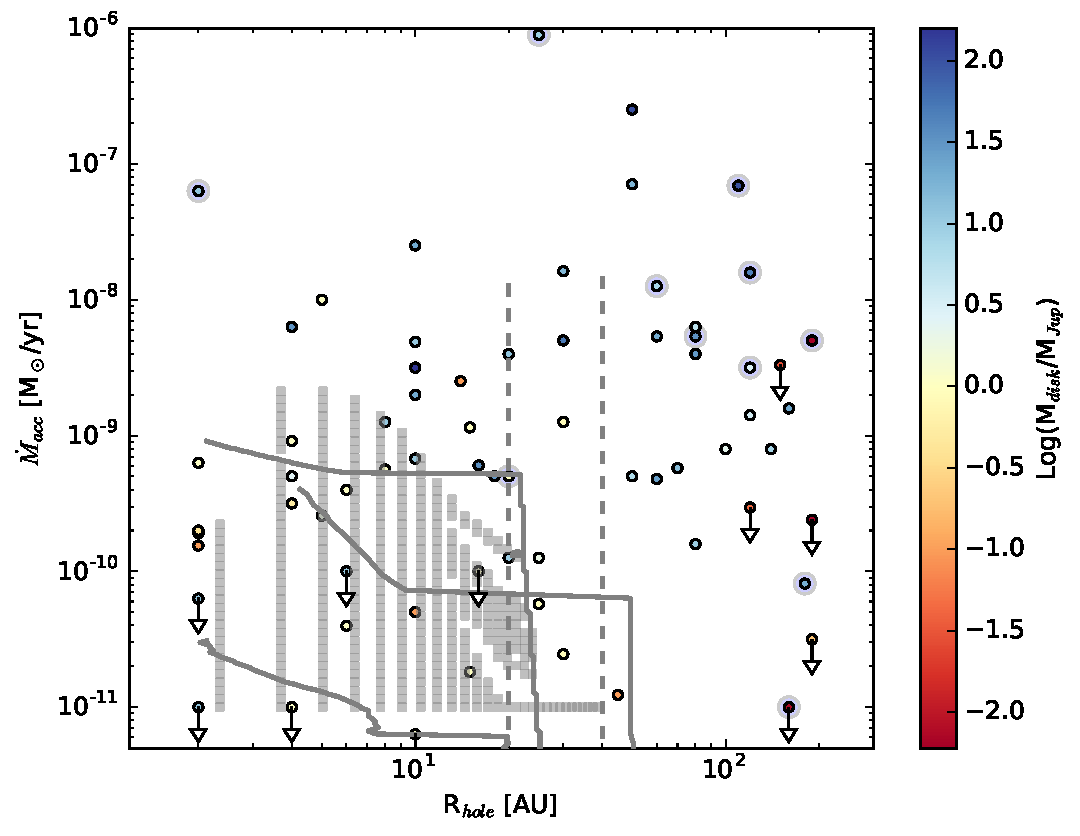
\includegraphics[width=0.75\textwidth]{figures/Macc_Rhole_Mdisk.pdf}}
\caption{\label{fig-macc-rhole-mdisk}
  Mass accretion rate versus hole size for known transition
  discs (Ercolano \& Pascucci 2017, in preparation). Circles are for
  observed star-disk systems. The color-coding shows total disk masses
  estimated from SED fitting. Sources surrounded by a
  light blue circle have spectral types G and earlier. Grey squares
  are snapshots of EUV- plus X-ray-driven photoevaporating discs from
  Owen et al. (2011) while grey lines are evolutionary tracks for the
  same photoevaporating discs with an embedded giant planet (Rosotti 
  et al. 2013).} 
\end{figure}

Figure~\ref{fig-macc-rhole-mdisk} shows a collection of known accretion rates versus inner hole
radii for known TDs (Ercolano \& Pascucci, 2017, in preparation),
represented by circles. These are compared to photoevaporation model tracks from
Owen et al. (2011), grey squares, and the photoevaporation models plus giant planet
of Rosotti et al. (2013, 2015), grey lines. 
If stars of spectral type G or earlier (distinguishable by a light
blue circle in the figure) are excluded, about half of the global TD population consists of Type 1
discs. The formation of Type 1 TDs is generally well reproduced by
photoevaporation models (e.g. Owen et al. 2010, 2011a). The large accretion rates and large hole
radii of Type 2 TDs, on the other hand, are problematic for all 
photoevaporation models (e.g. Rosotti, Ercolano et al. 2013, 2015) or grain
growth models (Birnstiel, Andrews \& Ercolano 2012) to date, and the classical explanation is that
these objects may have instead been carved by dynamical interactions
with forming giant planets (e.g. Zhu et al. 2011). However, since the
current models based on the classic planet scenario also generally
fail to reproduce the Type 2 TD observations and 
their demographics (e.g. see Dong \& Dawson 2016),
a number of alternatives have recently been proposed which include magnetohydrodynamics
effects (e.g. Wang \& Goodman, 2016), dust evolution (Pinilla et
al. 2016) and inner disc asymmetries (Montesino et al 2016). 

\begin{figure}
\centerline{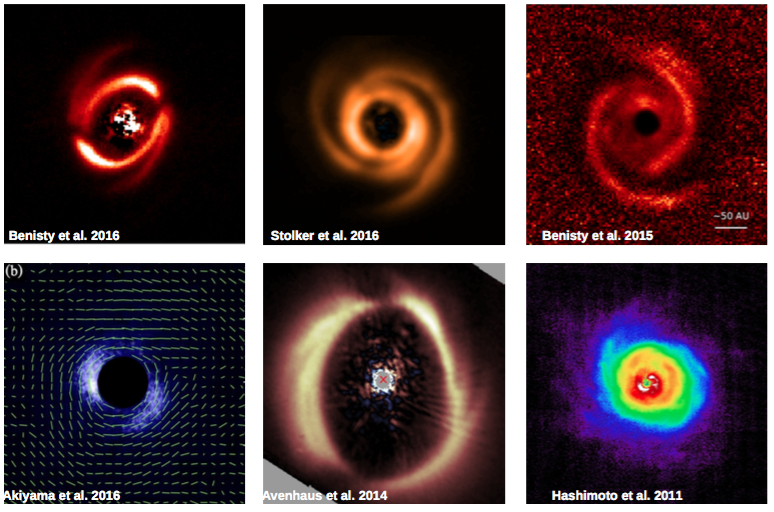
\includegraphics[width=0.75\textwidth]{figures/Type2TD_Scat.png}}
\caption{\label{fig-type2-scat}
  A gallery of scattered light images of Type 2 Transition Disks. 
\caphighlight{From left to right, top to bottom:} HD 100453, HD 135344b,
MWC 758, LkH$\alpha$ 330, HD 142527 and AB Aurigae.} 
\end{figure}

ALMA allows to measure the bulk of the molecular gas {\it
  directly}, showing than many Type 2 TDs have dense gas inside the
dust cavities (van der Marel et al., 2016), in agreement with the
planet scenario. {\color{red} IST THIS TRUE?? See Wang \& Goodman 2016}
Furthermore, spatially resolved observations of type
2 TDs have shown many bizarre features that are
not generally seen in primordial disks. For instance, they
  often display a huge dust ring (e.g.~Casassus et al.~2013)
  which is sometimes strongly lopsided (e.g.~van der Marel et al.~2013). The currently favored interpretation is that we see a
  key process of planet formation in action here: the mechanism of dust
  trapping in pressure maxima. Another spectacular kind of features often
  seen in TDs is spiral waves similar to those seen in galaxies
  (e.g.~Muto et al.~2012, Benisty et al. 2015, Wagner et al. 2015). Their origin is currently not
  understood, and trying to understand their physics may teach us about
important processes taking place in these discs. One interesting new
scenario, for example, was proposed to explain the bright ring of scattered light of
HD 142527 which has two dark spots on roughly opposite sides (see Fig.~\ref{fig-type2-scat}). Marino
et al. (2015) suggest that the shadows cast by an inclined small inner
disk could explain the location of the spots, implying that HD 142527
is an "inclined disc inside a disk". In that case, Montesinos et
al. (2016) claim that two shadows on opposite sides of the
bright rim may cause a brief pressure loss and be at the origin of the
m = 2 spiral waves. If confirmed this scenario opens a pandora of new
physical questions as to how could the inner disc have a different
rotation axis as the outer one?  \\

%{\bf What can we learn about Planet Formation from TDs? }\\
\subsection{What can we learn about Planet Formation from TDs? }

Both types of TDs can provide complementary information about the
planet formation process, if the observations can be interpreted
within a comprehensive theoretical framework. Type 1's
can inform us over the disc dispersal mechanism, which influences the
physical conditions in the disc at the time of planet formation and
migration. Type 2 TDs, if indeed formed by dynamical interactions with
giant planets are direct witness of the planet formation
process. Importantly, all disc-destruction mechanisms essentially `open up' the
  disc, so that we can peek inside to see its inner workings, and see
  processes of planet formation in action. TDs therefore
  have the unique potential of unveiling key aspects of the planet formation
process.

As mentioned above, as well as disc morphology, the interplay between disc evolution and
dispersal and the planet formation process, of which both types of TDs
are a
by-product, is apparent on many other
 levels. For example the lifetimes of protoplanetary discs (a few
Myrs) are comparable to the timescales for planet formation via the core
accretion model. This highlights the relevance of studying discs at the end
of their lives (i.e.\ TDs), and highlights the importance
of the disc dispersal mechanism (e.g. photoevaporation) which sets the
physical conditions in the disc at the time of planet formation. 
At the same time the similarity in the timescales for disc dispersal
and planet formation may also hint at the possibility that the planet
formation process plays a part in the final dispersal of the discs
(e.g. Rosotti et al. 2013, 2015). 


\begin{figure}
\centerline{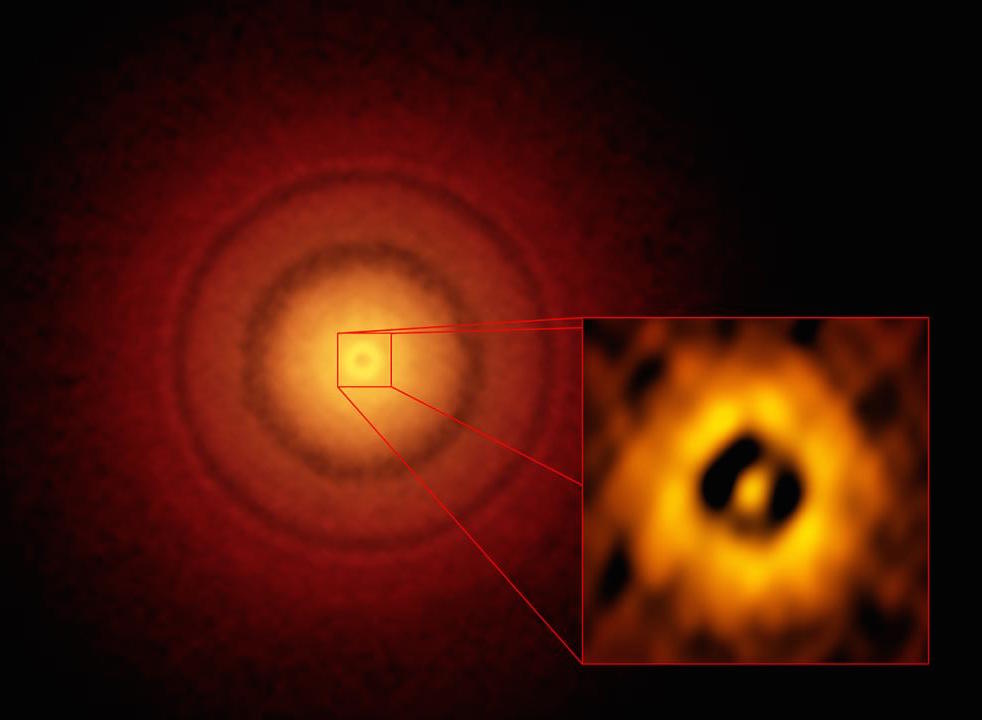
\includegraphics[width=0.45\textwidth]{figures/twhya.jpg}
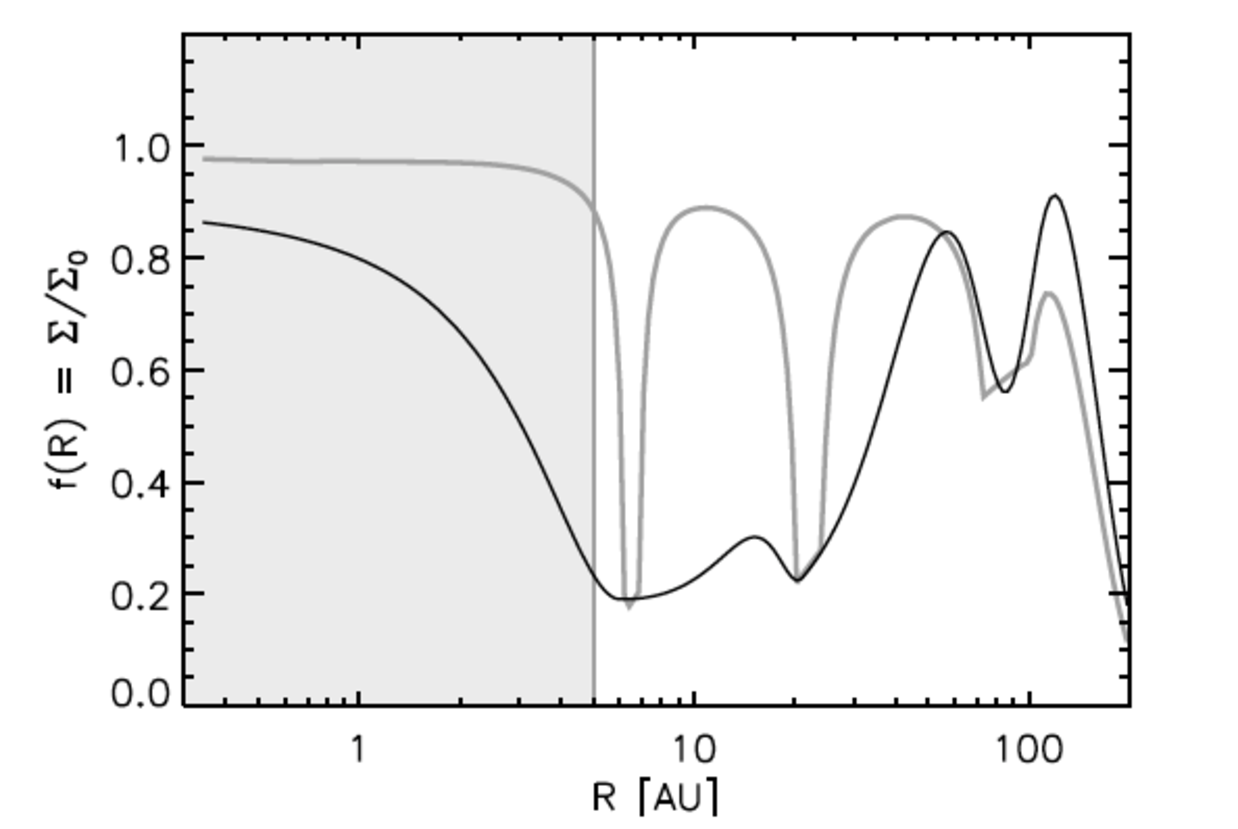
\includegraphics[width=0.5\textwidth]{figures/vanboekel.pdf}}
\caption{\caphighlight{Left:} ALMA image of the disk around the young,
  Sun-like star TW Hydrae. The inset image (upper right) zooms in on
  the gap at 1~AU . \caphighlight{Right:} Comparison between the derived radial surface density
depletion factor (f(R), black curve) from van Boekel et al. (2016) and an implementation
of the model of Duffell (2015) with three planets, approximately
matching the depth of the gaps (grey curve). The innermost disk
regions that are not well probed by the observations are masked. } 
\end{figure}


The recent ALMA image of the disc around the young solar-like star TW~Hya is a prime example of a disc showing hints of
planets orbiting at tens of AU,  co-existing with a inner gap at 1~AU
which could have been 
recently created by photoevaporation (Ercolano et al. 2017). The ALMS image
is shown in the lef panel of Figure~\ref{fig:twhya} and was obtained by
a team including members of this Research Unit (Andrews, et
al. 2016). However both the existence of planets and the
photoevaporated gap remain speculative at present. As shown in the
right panel of Figure~\ref{fig:twhya}, current planet-disc interaction
models fail to reproduce the shape of the gaps as obtained from
scattered light observations taken with SPHERE (van Boeckel et
al. 2016). Furthermore, while several spectral line observations exist
for TW Hya, the photoevaporation models do not yet have the predictive
power to directly measure the mass loss rate in the wind from
them. Until that becomes possible, even the nature of the gaps and rings
the nearest and best studied of all (pre-)Transition Discs, remain
uncertain. 

 The inside-out dispersal of
protoplanetary discs, forming TDs, is also an important
factor to consider when studying the final architecture of
exo-planetary systems. While planet migration is necessary to explain
(e.g.) the presence of large planets close to the central star, the
so-called ``hot Jupiters'', this process alone cannot explain the pile-up and
deserts in the semi-major axis distribution of exoplanets (see also
Chatterjee \& Tan, 2014, 2015). An
additional planet-parking mechanism is required, which may be provided by (e.g.)
photoevaporation which opens a gap in the disc, forming a TD and
stopping further planet migration (e.g.\ Alexander \& Pascucci 2012; Ercolano \& Rosotti
2015).

 %
%\vspace{1em}
%\noindent {\bf Why is a Research Unit on TDs needed Now?}\\
\subsection{Why is a Research Unit on TDs needed Now?}
%
 From the above argumentation it becomes clear that TDs are
  unique laboratory experiments created by Nature that allow us to test and
  update our understanding of disc structure and evolution as well as planet
  formation processes on the small scale (dust growth and dynamics) and
  large scale (planet assembly and planet-disc interaction). 

New observational facilities including ALMA and VLT-SPHERE are revolutionising our view of
TDs. We are now starting to obtain extraordinarily detailed images of these objects at infrared and
millimetre wavelengths. While the new observations are fundamental to pin down many important
characteristic of the dust and gas density distribution in the bulk of
these discs or in their cavities, the disc atmospheres and winds, which bear the signature of the dispersal mechanism, are
best traced by high resolution observations of emission line profiles. As well as a number of surveys
which are in course on the VLT in the optical, the mid-infrared region will also see a wealth of new
data with the upgrade for the CRIRES instrument, which has an an expected delivery date of 2019.
A solid theoretical framework is thus urgently needed in order to interpret the new/future
observations and decode the message encrypted in the spectral and continuum emission of
TDs. The new models developed in this project are exactly what is needed at this stage.
Furthermore, models for the formation and evolution of planetary systems are reaching new
levels of complexity, but they remain limited due to the current uncertainties in the boundary/initial
conditions inherent to uncertain disc physics.

  Now that the
  era of high-resolution optical/infrared and (sub-)millimetre imaging is
  under way and starts revealing complex structures in these discs, the time
  is ripe for a concerted theoretical/numerical modeling counterpart to
  these observational studies. To be able to understand the observed
  features and statistics of TDs, this effort must combine the
  theory of disc structure, evolution and destruction with dust growth and
  dynamics, as well as with planet-disc interaction and dynamics. It can
  therefore not be done in a single or a set of DFG individual proposal, but
  requires a concerted, closely knit small network of projects involving
  several teams, covering the key observational and theoretical
  skills. To make the link to the observations of these disks, 
  which are typically done in scattered light (optical/IR), dust thermal
  emission (sub-millimetre) and molecular rotational lines (sub-millimetre),
  our effort has to also include modeling of disc chemistry and radiative
  transfer, as well as team members with detailed understanding of the
  observations and their limitations. This is the motivation of the research
  group we propose here.


\section{Contribution of this team to the field }
%
%The process of planet formation cannot be observed directly and
%therefore theories of planet formation theories are built using the
%indirect constraints provided by the observable consequences of
%planet formation on the structure and evolution of protoplanetary
%discs, in particular TDs. Indeed recent ALMA
%observations of discs have provided many surprises posing new
%challenges to existing theories of (e.g.) dust aggregation and
%retention, protoplanetary disc dispersal and planet-disc interactions
%and migration. One of the most famous examples is the image of the
%relatively young disc around HL Tau, which already shows a multiple
%ring structure, speculated to be due to planets forming. Transition
%discs are indeed the best laboratories to study these processes,
%which are all likely to play a role in their formation. 
%On the theory side our team includes
%dynamicists, experts in radiative transfer and astrochemistry, who are
%committed to exploit the synergies of the team to provide a holistic
%approach to understanding planet formation and disc evolution, via the
%study of TDs and their formation. \\

Our team is composed by theorists and observers, who have all
contributed significantly to the state-of-the art of the field today. 
On the theory side our team includes
dynamicists, experts in radiative transfer, dust evolution and astrochemistry, who are
committed to exploit the synergies of the team to provide a holistic
approach to understanding planet formation and disc evolution, via the
study of TDs and their formation. \\

{\it Speaker: }{\bf Prof.\ Barbara Ercolano (LMU)} has been studying the link between high
energy radiation from the central star and disc evolution and
dispersal (e.g. Ercolano et al. 2008a, 2009; Owen, Ercolano et
al. 2010, 2011, 2012). Before Ercolano et al. (2009), the importance
of X-ray radiation from the central star on the dispersal of discs had
not been recognised. This process is now accepted as one of the major
player for disc dispersal, hence setting the timescale for planet
formation. The models have been tested against observables
(e.g. Ercolano et al. 2010; Owen, Scaife \& Ercolano 2013; Koepferl,
Ercolano et al. 2013; Ercolano, Koepferl et al. 2015), producing
several successes, but also opening new questions (e.g. Ercolano \&
Owen 2016), such as those to be
approached as part of the projects proposed here. Prof. Ercolano and
her team have also investigated the effects of X-ray irradiation on
the final parking radius of exoplanets (Ercolano \& Rosotti, 2015), as
well as on the intrinsic (Ercolano \& Glassgold 2012, Mohanty,
Ercolano \& Turner, 2013) and observed
accretion properties of protoplanetary discs (Ercolano et
al. 2014). With the work of Rosotti, Ercolano et al. (2013, 2015) the
interaction between planet formation and photoevaporation was first
taken into account, in an attempt to match TDs
statistics. Together with Prof. Testi, she recently published a Letter
showing that the innermost gap in the closest planet-making disc to
Earth, TW Hya, could be the first photoevaporative gap
imaged. Prof. Ercolano is also the main author of the dust RT and 
photoionisation code {\sc mocassin} (Ercolano et al. 2003, 2005,
2008b), which is one of the main tools
used for the subpojects in area B. This code includes X-ray processes
and was recently ported to Voronoi grids (Hubber, Ercolano \& Dale,
2016) For the development of {\sc
  mocassin} Prof. Ercolano received the Royal Astronomical Society
Fowler Prize for early career achievements in 2010 (https://www.ras.org.uk/news-and-press/157-news2010/1713-ras-honours-outstanding-astronomers-and-geophysicists). \\

{\it Co-Speaker:} {\bf Prof.\ Cornelis Dullemond (ZAH)} is an expert in modeling the radiative transfer in protoplanetary
disks, to compute the (vertical) disc structure and the disk's appearance as seen
by observational facilities. He is the author of the popular open source RADMC-3D 
radiative transfer modeling package, which he and his team employ to study
protoplanetary disks, and linking models to observations at infrared and submillimetre
wavelengths. He develops new methods for disc modeling, and has been involved
in the development of new radiation hydrodynamics modules for the PLUTO code
(Kuiper et al. 2010) and ZEUS (Ramsey et al. 2015). His group has also played a
leading role in global disc modeling with dust growth and drift (e.g. Brauer et al. 2008;
Birnstiel et al. 2010), the subsequent planetesimal formation (e.g. Drazkowska 
\& Dullemond 2014), and the link between the disk/dust models and millimetre
and infrared disc observations (e.g. Pinilla et al. 2014; van der Marel et al. 2013;
Kataoka et al. 2015). A key theme in the research of Dullemond's group is the study 
of physical processes and how we can constrain them with observations. The
group often develops its own methods of computation and own codes to implement
the new physics in existing models, and thereby opening new
directions. \\

{\it Co-PI:} {\bf Prof.\ Wilhelm Kley (University of T\"ubingen}) is an expert in computational astrophysics with emphasis on the
planet formation process, starting from the growth of small dust grains all the way
to full grown planets. The numerical methods developed and used in his group range 
from molecular dynamics, smoothed particle hydrodynamics (SPH) and grid-based 
magneto-hydrodynamics (MHD) including radiative transport. These methods will be used
in the theoretical modeling within the Research Group.   
One focus of his research has been on the important planet-disk
interaction. Through multi-dimensional (2D and 3D) radiation hydrodynamical simulations
his group demonstrated the possibility of strongly reduced or even outward migration
(Kley \& Crida, 2008; Kley, Bitsch \& Klahr, 2009). Recently, models for the origin of the
circumbinary planets have been presented (Kley \& Haghighipour, 2014). Here, longterm models of
disks in the presence of a central binary have been simulated and the motion of an embedded
planet has been followed. Concerning the main focus of this research group, M\"uller \& Kley
(2013) constructed time-dependent hydrodynamics models of transitional disks induced by the
presence of a single planet. Specifically, the models investigated the amount of gas flow past
the planet into the inner hole as a function of the planet mass, disc
parameter and stellar irradiation. With Picogna \& Kley (2016)
significant advances were made in the understanding of the dust phase
response to planet-disc interactions. \\

{\it Co-PI:} {\bf Prof.\ Paola Caselli (MPE)} 
% moved to MPE as Director of the new Centre
%for Astrochemical Studies in April 2014, after spending almost seven
%years as Professor of Astronomy at the School of Physics and Astronomy
%at the University of Leeds, UK. She
is an expert on astrochemical
modelling and observations of the earliest phases of star and planet
formation. She has made important contributions on the chemical structure
of pre-stellar cores (within which future stellar systems form.)
%finding that: CO molecules are almost completely ($>$90\%) frozen onto
%dust grain surfaces in the central few thousand astronomical units
%(Caselli et al. 1999), thus thick CO-ice mantles are predicted to be
%present just before a protostar is born; deuterated molecules are the
%best diagnostic tools of the physical properties of the central
%regions, the future stellar cradles (Caselli et al. 2002, 2008;
%Crapsi, Caselli et al. 2005, 2007); the tenuous UV field produced by
%cosmic-ray impacts with H$_2$ molecules plays an important role in
%producing water vapour and regulating the gas-solid phase in these
%dense and cold phases preceding star formation (Caselli et al. 2012);
%a dust opacity increase toward the pre-stellar core centre is needed
%to reproduce the observed temperature drop (Keto \& Caselli 2010),
%suggesting that dust grains have already started to coagulate;
%quasi-static contraction best reproduces the observed molecular line
%profiles toward one of the best studied pre-stellar cores (Keto,
%Caselli \& Rawlings 2015), showing in this case that the dynamical
%evolution toward protostellar birth is a slow process, maybe regulated
%by the action of magnetic fields in partially ionised media. 
She is
now focusing on the link between molecular clouds and protoplanetary
disks using high angular resolution observations, hydro- and
magneto-hydrodynamical simulations, which incorporate various degrees
of chemical complexity, and radiative transfer codes. She is
interested in understanding the effects of different initial
conditions in the physical and chemical evolution of protoplanetary
disks. Already published work in this field include the chemical
structure and ALMA observability of a self-gravitating disc orbiting
around a protostar which will likely evolve into a future F-type main
sequence star (Ilee et al. 2011; Douglas et al. 2013) as well as the
chemical evolution of a self-gravitating disc surrounding a
protosolar-type star (Evans et al. 2015). 
%; all this work on young disks
%has been done with students and former students from the University of
%Leeds, partially funded by the ERC grant PALs 320620).
%Self-gravitating disks are thought to be important during the earliest
%phases of protostellar evolution, although their existence still need
%to be confirmed with ALMA.  
Using non-ideal MHD simulations of contracting dense cloud cores, she recently found that the disappearance of very small grains (VSGs), due to accretion onto larger grains, enables the formation of protoplanetary discs (Zhao, Caselli et al 2016). This is due to the fact that VSGs dominate the coupling of the bulk neutral matter with magnetic fields, thus allowing an efficient loss of angular momentum (via magnetic breaking) in regions where protoplanetary discs should form. Together with plasma physicists, she also started a detail study of dust grain charging and its effect on dust coagulation (Ivlev, Padovani, et al 2015).
Her expertise on basic astrochemical
processes will be applied to the available and future dynamical models
of transition disks. \\

\textit{Co-PI:} \textbf{Dr.\ Tilman Birnstiel (LMU starting in 02/2017)} has been
studying the crucial early stages of planet formation by simulating growth,
destruction, and global transport processes in disk
\citep[e.g.][]{2010A&A...513A..79B}. While some of the transport processes have
been proposed in the 70s, they were often neglected as they seemed incompatible
with observations of disks. Birnstiels models were the first to show, that these
processes are not only consistent with many observations but are necessary to
explain and understand the evolution of disks \citep{2010A&A...516L..14B}. His
models successfully explained or even predicted observed signatures of growth
and transport processes: the spectral index behavior predicted in
\citet{2010A&A...516L..14B} was observed in \citet{2012ApJ...760L..17P},
\citet{2016A&A...588A..53T} and others. Small scale pressure traps were needed
to explain the integrated continuum emission properties of disks
\citep{2012A&A...538A.114P}, which strikingly resemble the observations of
\citet{2015ApJ...808L...3A} and \citet{2016ApJ...820L..40A}. Sharp dust edges in
protoplanetary disks as predicted in \citet{2014ApJ...780..153B} are now seen in
almost every observation that has high enough resolution and sensitivity
\citep[e.g.][]{2016ApJ...820L..40A,2013A&A...557A.133D}. Lately, for the first
time, signatures of his predicted effect of dust accumulation inside the water
snow line \citet{2010A&A...513A..79B} have been detected in
\citet{2016Natur.535..258C}. His models have substantial impact on the further
evolution of planet formation via a range of effects: they provide the
``pebbles'' for pebble accretion, they predict how the planet forming material
is redistributed within the disk, they determine the continuum opacity and
therefore the temperature and observational appearance of disks, they feed the
planetesimal formation factories and transport key volatile species along the
way and finally they provide the surface area for chemical reactions that determine the
chemical composition of the disk. To investigate these links to planet formation
and to the disks chemical composition, he has been awarded an ERC starting grant
that starts in March 2017, is hosted at the LMU, and perfectly complements
the goals and work plan of this research group proposal.

 On the observational side our group includes experts on the
 observations of young stellar objects, transition discs, initial stages of
 planet formation and planet disc interactions. Our observational
 team is experienced with state-of-the art observational facilities
 including \todo{sentence ends abruptly}.\\

{\it Co-PI:} {\bf Prof.\ Leonardo Testi (ESO)}, \todo{Check Prof.~Title (I don't
mind but in Germany they are pretty touchy when it comes to titles.} has accumulated years of expertise
in the observation and analysis of young stars and their protoplanetary
discs at infrared and millimetre wavelengths. He has investigated the initial stages of planet formation via
extensive studies of properties and evolution of dust in discs (e.g. Testi et
al. 2003, 2014). With his group at ESO has completed the first large observational surveys for dust growth
in disks (Ricci et al. 2010ab) and has developed the first self-consistent analysis tool to constrain dust properties
as a function of radius in discs (Banzatti, Testi et al. 2011, Trotta,
Testi et al. 2013, Tazzari, Testi, Ercolano et al. 2016). His group also developed the methodology to perform accurate measurements of the photospheric properties and accretion rates from broad-band XShooter spectra (Manara, Testi et al. 2013) and applied it to study the correlation between disc properties and mass accretion rates in young stars with disks (Manara et al. 2016).
His current role as European ALMA Programme Scientist at ESO
puts him in a very favourable position to lead an effort here in
building a systematic catalogue of the available ALMA observations and help with the interpretation of these data in terms of
the models. The new observational
campaigns that we foresee for phase 2 of the Research Unit will also
strongly 
benefit from his guidance. \\

{\it Co-PI:} {\bf Prof.\ Thomas Preibisch (LMU)}  has many years of experience in the
fields of stellar X-ray astronomy and infrared observations
of young stellar clusters.
He was deeply involved in the
Chandra Orion Ultradeep Project (COUP;  see Preibisch et al. 2005),
the Chandra Carina Complex Project (CCCP; see Preibisch et al.~2011),
and numerous other projects where
the identification of the X-ray sources with optical
and infrared counterparts was a crucial step for the studies
of the relation between the X-ray properties and the stellar/circumstellar
properties of the young stars. He has also performed several large-scale surveys of star forming
regions in the near-infrared (e.g., Preibisch et al.2011,
Preibisch et al. 2014)
and far-infrared regime (e.g, Preibisch et al. 2012)
with the aim to identify protostars and study disk-bearing young
stellar objects.\\

{\it Collaborator:} {\bf Prof.\ Thomas Henning (MPIA)}  is co-I
on the VLT SPHERE disk programme and therefore has prime access to
high-contrast high-resolution scattered light images of Transition
Discs. He has been involved in many protoplanetary disc projects, both
observationally and theoretically. He is co-author of the Klahr \&
Henning (1997) paper predicting the role of dust trapping in vortices
in protoplanetary disks, something which has recently beensie 
observationally confirmed in transition disks. His involvement in this
Research Unit will be through discussions/collaboration on the
modeling and through comparison with the observations. \\

{\it Collaborator:} {\bf Prof.\ Ewine van Dishoeck (MPE/Leiden)}
is one of the founders of ALMA observatory. In recent years her group
has focussed on studying Transition Disks with ALMA. In 2013 her team
published the first strong evidence, based on ALMA data, for a
dust-trapping vortex in the Transition Disk Oph IRS 48 and in 2016 her team found wide-spread
 evidence for dense molecular gas inside dust cavities. She has been
involved in many protoplanetary disk studies, both observationally as
well as from an astrochemical perspective. Her involvement in this Forschergruppe
will be through discussions/collaboration on the modeling and through comparison with
 observations of the gas surface density structure.\\


\section{Scientific Objectives}

Planet formation and disc evolution feed back on each other. Indeed
the formation and migration of planets in protoplanetary discs is
clearly affected by the structure and the physical properties of the
disc itself (e.g. D\"urmann \& Kley, 2016; Ercolano \&
  Rosotti, 2015, to cite only a few of the works coming from our team). The
structure and evolution of the disc, however, can be also deeply
influenced by the planet formation process, as demonstrated by our
recent calculations (e.g. Rosotti et al. 2013, 2015). 

This has important consequences both in the interpretation of the observed
exo-planet properties (eg. size and semi-major axis distributions) as
well as in the interpretation of the disc structures, which are often
used as tell-tale signs for planet formation, as in the case of the
TDs. Our understanding of how the two processes
influence each other is however still at incomplete. A  more
complete picture of planet formation and disc evolution is thus only
possible with an interdisciplinary aimed at obtaining more holistic answers to
a number of important questions. 

Some of the key questions that will be addressed in the proposed
Research Unit and the immediate objectives which relate to them are
described in what follows. 

\subsection{First Main Question: How can we use TDs as direct witnesses of the planet
  formation process?}
Which TDs are carved by planets and which are a result of disc evolution? \\ What do the complex shapes of TDs (rings, blobs, spirals) teach us about the physical and
dynamical processes taking place in protoplanetary disks?\\ How does
dust evolve and travel within discs to form planet(esimal)s?

To answer these questions we will use the following approach: 

\begin{itemize}
\item{\it Investigate observationally the accretion properties
  and the distributions of dust and gas in the discs and winds of
  primordial compared to transition objects.} To this aim a systematic catalogue of observations will be built, which will provide the constraints to the modelling efforts described below. 
\item{\it Dust trapping and growth in TDs.} Dust and
gas hydrodynamical models of discs with and without cavities will be produced to match the
constraints from the observations, these will put constraints onto the
planet-disc interaction and photoevaporation models described below. 
\item{\it Planet-disc interaction models with photoevaporation
  and dust trapping.} These models will aim at reproducing
observations of (mainly) Type 2 TDs, including their accretion properties, to pin down the formation mechanism of the observed structures. 
\end{itemize}



\subsection{Second Main Question: How can we use TDs to learn about the disc dispersal
    mechanism?}
 What are the mass loss rates of the disc wind and
  what parameter space in the TD demographics can thus be reproduced
  by photoevaporation?\\ What are the dust and gas surface density
  distributions in TDs and how can they be
  explained?\\How does the high-energy emission from the central
  star regulate disc accretion and dispersal, leading to the formation
  of different types of TDs?

To answer these questions we will use the following approach: 

\begin{itemize}
\item{\it Determine the mass loss-rates of photoevaporative winds
  to pin down the mechanism producing Type 1 TDs.} To
this aim appropriate wind diagnostics need to be identified via
chemical modelling of  photoevaporative winds, comparing primordial to
TDs. Existing archival observations will be used at first to compare
with the models and a new observing campaign with ALMA will be
devised, perhaps spilling into the second funding period of the Research Unit.
\item{\it Determine the dominant dispersal mechanism.} We will
use the archival observations and the models from item 2.1 to analyse
an initial sample of discs, the final statistics will be achieved
however in the second funding period, where a population synthesis of
(Type 1) TDs will be attempted.
\item {\it Close the loop using mass loss rates, central star
  properties and accretion measurements to calibrate models.}  At this
point the models will have significantly less free parameters and can
be used to extract the initial conditions for planet formation
(e.g. mass, turbulence in evolved discs). This will make use of the new state-of-the
art simulations and a homogeneous sample of accretion rates and central
star properties including X-ray data. 
\end{itemize}

\section{Work plan}
%\vspace{1em}\\

%\noindent{\bf \em Overview over the Research Unit}\vspace{0.8em}\\
\subsection{Overview over the Research Unit}
%
The main goal of this Research Unit is to understand the morphology,
spectroscopy and demographics of TDs, in order to answer
basic questions about the planet formation process. We propose a
four-pronged coordinated effort which includes (A) Observational
studies; (B) Disc dispersal models; (C) Dust physics; (D) Planet-disc
interaction models. The division in subfields is not strict and is
only given here in the aid of clarity. Subfields often overlap and/or
feed back on each other, highlighting the need of strong
collaborations as proposed here. The observations will provide the
constraints to be simultaneously met by models developed in the other
areas. Our team is supported by several external collaborators in particular
Prof. T. Henning (MPIA) and Prof. E. van Dishoeck (Leiden/MPE) have
agreed to take an active part in our project. The theoretical models in the three theory subfields require
expertise in hydrodynamics, astrochemistry, dust evolution and
radiative transfer, which is available in our team. The specific
projects in each area, the support required and the respective members
of the team are summarised in the table below. 
\vspace{1.5em}

\noindent
\begin{tabular}{p{1cm}p{8cm}p{2.0cm}p{3.9cm}}
\hline
{\bf\AreacolA A} & {\bf\AreacolA Observations} & & \\ 
A1 & ``Solids and gas evolution in disks: observational constraints'' & 2 PhD & {\em Testi, Ercolano, Preibisch}\\
A2 & ``New constraints about disc-dissipation processes from the relation between accretion and X-ray activity'' & 1 PhD & {\em Preibisch, Ercolano, Testi}\\
\hline
{\bf\AreacolB B} & {\bf\AreacolB Disc dissipation and chemistry} & & \\ 
B1 & ``The radiation-hydrodynamics of photoevaporative winds with chemistry'' & 1 Postdoc & {\em Ercolano, Caselli}\\
B2 & ``Astrochemistry in the atmosphere and winds of photoevaporating discs '' & 1 Postdoc & {\em
                                                              Caselli,
                                                              Ercolano,
                                                              Ivlev}\\
\hline
{\bf\AreacolC C} & {\bf\AreacolC Dust physics} & & \\ 
C1 & ``Trapping the dust: Planet formation 'hotspots' in TDs'' & 1 PhD
                               & {\em Birnstiel, Dullemond, Kley}\\
C2 & ``Gone with the wind: Dust entrainment in photoevaporative winds
     from realistic underlying grain distributions "& 1 PhD & {\em
                                                              Ercolano,
                                                              Birnstiel,
                                                              Dullemond}\\
\hline
{\bf\AreacolD D} & {\bf\AreacolD Planet-disc interactions} & & \\ 
D1 & ``Transition disks and planetary systems''' & 1 Postdoc & {\em Kley, Dullemond}\\
D2 & ``Origin of complex non-axisymmetric structures in type 2
     Transition Disks "& 1 Postdoc & {\em Dullemond, Kley}\\
\hline
\end{tabular}
\vspace{1.5em}

Figure 2 shows schematically the direct links between the listed sub-projects, which provide the foundation for the Phase 2 study. Details about the major links between sub-projects are summarised in the next Section. 

\begin{figure}
\centerline{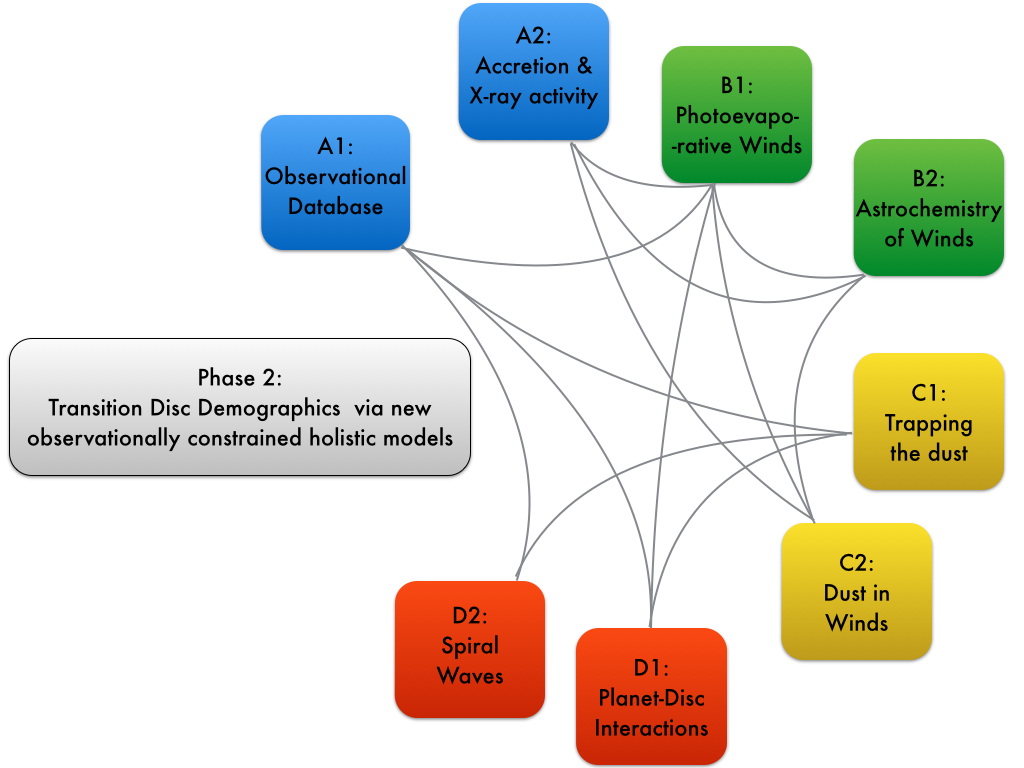
\includegraphics[width=13cm]{figures/dependency2.jpg}}
\caption{A diagram showing the links between the various
projects. See text for detail.}

%\vspace{2em}\mbox{}\\
%\centerline{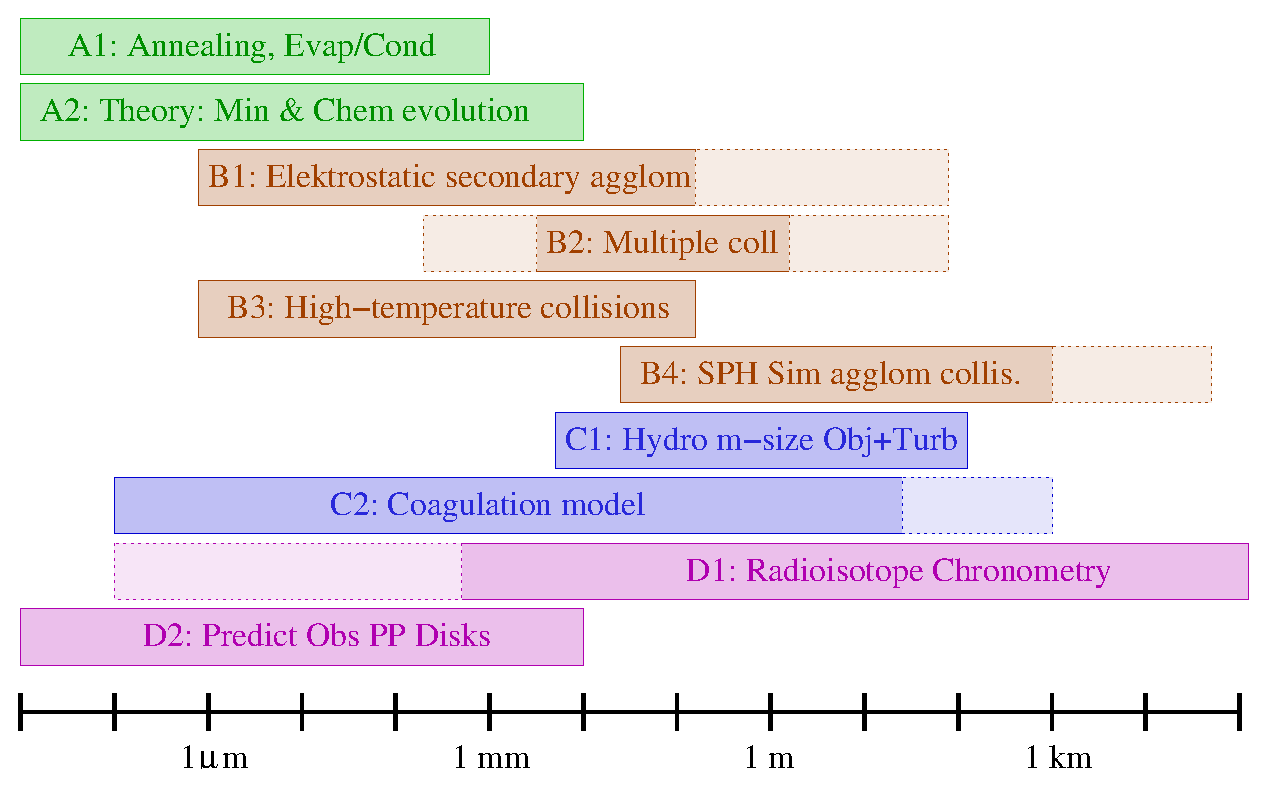
\includegraphics[width=16cm]{sizebar.eps}}
%\vspace{1em}\\
%Fig 2: A diagram showing the coverage
%of the size-range between sub-micron dust particles and
%multi-kilometer-sized planetesimals.
\end{figure}

\vspace{1.0em}


%
\noindent\underline{{\bf\AreacolA Area A: Observations}}\\
\noindent The projects in this area both aim at obtaining
observational constraints on the dust and gas properties of
protoplanetary discs and their central stars. Project A1 focusses on
collecting and analysing existing ALMA data and complementing those
with additional ALMA, VLA and high-contrast infrared imaging observations. 
The aim is to characterize the content and properties of solids and gas in TDs 
and to compare with the demographical properties of evolving disk populations. 
Evidence for dust and gas evolution, including grain growth,
and planet-disc interactions will be characterised in order to provide
direct observational tests of planet formation and dispersal theories,
necessary to interpret the observational appearance of Type 1 and 2
TDs. The focus of project A2 is on the central star properties and
their relation to the accretion properties of the disc, which may be
modulated by the disc dispersal mechanisms that lead to the formation
of TDs. While both of these projects have self-contained aims, they
will also provide the observational goalposts for the theoretical
investigations of all projects in areas B, C and D, and indeed a
legacy for future theoretical studies of this kind also by other
groups.  

%

%\vspace{1em}\\

%\pagebreak[4]

\
\mbox{}\vspace{1em}\\
\noindent\underline{\bf\AreacolB Area B: Disc dissipation and chemistry }\\
\noindent The main objective of the projects in this area is to
determine the mass loss rates in disc winds, and constrain once and
for all the disc dissipation mechanism, leading to the formation of
Type 1 TDs. This is crucial to interpret the observed Type 1
demographics. We will perform quantitative spectroscopical modelling
of disc winds, identifying and using new wind diagnostics, in
particular comparing primordial and TDs. In project B1 we will develop
the most comprehensive radiation-hydrodynamics models of
photoevaporative disc winds to date. The physics beyond the X-ray
heated layer will be accounted for for the first time. This will be
achieved by coupling our  (radiation-)hydrodynamics code, PLUTO, to an efficient 
chemical solver for a reduced network,
developed in project B2. Project B2 aims at producing a detailed astrochemical model of the
disc atmosphere and its wind. By means of radiative transfer
calculations a synthetic spectrum will be obtained to be compared with
state-of-the-art observation of spectrally revolved emission from
discs, particularly those with known cavities (TDs). The intensity and
profiles of emission lines tracing the base of the wind will allow us
to put constraints on the wind-launching mechanism, responsible for
the dispersal of the discs.  

Both projects will use existing and new observational
constraints coordinated in projects A1 and A2, and also provided by
our external collaborators. The dust 
content of the wind which is of prime importance for the chemical
modelling will be provided by project C2. Project D1 will inform us on
planet-disc
interactions which may help photoevaporation create gaps and holes at
earlier times and may cause 
strong asymmetries, yielding different streamline
architectures (see e.g. Rosotti et al 2013, 2015).\\ 

%
\mbox{}\vspace{1em}\\
\noindent\underline{\bf\AreacolC Area C: Dust Physics}\\
\noindent The dynamics and evolution of dust grains in discs is the
main subjects of this area. In project C1 we will study the growth and
trapping of dust grains at hotspots in TDs that may lead
to breaking through the meter-size barrier of radial drift, thus
allowing the formation of planetesimals. We will use (radiation
hydro)-dynamical modelling and dust coagulation models as well as 3D
radiative transfer tools. Furthermore, we will be able to use the
observational sample collected and analysed in project A1 to tackle
fundamental open questions on the first stages of planet
formation. This project will feedback and take inputs from the
photoevaporation modelling performed in project B1 and it will
eventually produce
the underlying dust distributions for project C2, which aims at
determining the dust content of photoevaporative winds. The latter
will make use of state-of-the art models of photoevaporating
primordial and TDs from project B1 as well as inputs for the dust distributions from
project C1, in order to constrain dust entrainment in the wind, which
is an important input to the chemical models in project B2. Finally,
project C1 would highly benefit from the setups and methods developed
in the more detailed models of Area D.\\ 


%\pagebreak[4]


\mbox{}\vspace{1em}\\
\noindent\underline{\bf\AreacolD Area D: Planet-disc interactions}\\
\noindent Projects in this area aim at constructing realistic
simulations of planet-disc interactions and studying the dynamical processes
leading to non-axisymmetric features in order to explain the wealth of new
and intriguing observations of TDs. The overarching goal is to use
these observation-constrained (from project A1) models to pin down
the important details of the disc interaction processes. This is of
fundamental importance to be able to disentangle the message about
planet formation which is locked in TDs observations. In particular
project D1 aims at significantly pushing forward the state-of-the art
of (radiation)-hydrodynamical models of gap-forming giant planets
embedded in discs including dust dynamics. 
This project will provide important inputs of
gas and dust density distributions for project B1, particularly informing about the
fate of dust grains at planet-gaps, which is also relevant to project
C1. Project D2 aims at explaining the surprising non-axisymmetric
structures recently observed with ALMA in a number of TDs, via
detailed hydrodynamical and radiative transfer models, which will also
account for realistic grain size distributions from project
C1. Studying the intriguing nature of these objects is likely to
provide important insights on planet-disc interaction processes, thus
enabling us to use these discs as proxies for planet formation.  \\ 

%\mbox{}\vspace{1em}\\
%\noindent{\bf \em Future perspectives}\\
\subsection{Future perspectives}
%
While all sub-projects presented here are self-contained and will
provide specific intermediate science products, the major strength of this program is the collaborative
work to produce a holistic picture of protoplanetary disc evolution
and dispersal, which through the study of TDs can be used
to inform us on the planet formation process. At the end of Phase 1 of
the Research Unit all theoretical models will have been significantly
improved to allow a much more realistic approach to match the
observational constraints. At the same time the systematic analysis of
the existing observations and the collection of new data will have also
provided a much clearer picture of disc structures, as possible planet
formation signatures. At the end of Phase 1 our team will be then
perfectly posed to perform the most advanced simulations of individual
objects, but also and perhaps more importantly, we will be able to
tackle the issue of demographics of TDs. Via population
synthesis models of TDs including disc dispersal, planet formation, dust
evolution, some simplified chemistry and radiative transfer, we will
be able for the first time to use discs to make predictive models of
planet formation and evolution to match existing exo-planet
statistics. 

We thus foresee a two-pronged approach in Phase 2: 

i) Detailed modelling of individual objects.\\
This will follow mainly from the joint work of areas A (in particular
A1) and D, and will target mainly Type 2 TDs. The insights gained in
Phase 1 of the Research Unit will allow us to construct tailored
models of planet-disc interactions to explain specific observations of
Type 2 TDs (not necessarily obtained by our group). The tailored
models will allow us to decode the message in the many interesting new
features highlighted already by spatially resolved observation, which,
by the beginning of the second funding period, will have surely
delivered more surprises.  

ii) Statistical distributions/demographics of Type 1 TDs. \\
The work carried out in Phase 1 in areas A, B and C will have resulted
in the most advanced disc dispersal models, which would have also been
calibrated for important quantities with direct observations. We will
use these models to construct population synthesis of Type 1
TD demographics (e.g. inner hole radius vs accretion
rate), to compare with available surveys in individual clusters.  
This will be a very strict, direct test of our disc models, and will
allow us to predict realistic initial conditions in a disc population at the
time of planet formation and migration, which are fundamental inputs
for planet formation models (the latter are however beyond the scope of this
proposal).  

It is inappropriate at this stage to design a more detailed program
for a potential Phase 2 of the Research Unit. As well as depending on
the outcome of our Phase 1 projects, the exact focus of a potential
extension would depend on the developments of the field as a
whole. Some general ideas go in the direction of providing the basis for more detailed chemical
and physical evolution of Solar-Nebula-type discs, needed to gain a
better understanding of the Solar System origin and composition,
including the large variety of minerals and organics found in comets
and meteorites. 
\vspace{0.8em}

%\noindent{\bf \em Research Environment of the Research Unit}\\
\subsection{Research Environment of the Research Unit}

The new young Research Unit members will be welcomed in a stimulating
environment, where complementary research programs are being carried
out at all of the institutions involved. 

At the LMU, Prof. Birnstiel's group (funded by an ERC starting grant)
will focus on several aspects of dust evolution in planet-forming
disks, with the aim of pushing the state-of-the-art of what is
possible with current codes. Prof. Preibisch's group can provide
support on observational aspects of high energy radiation from young
stars. Prof. Ercolano's group comprises experts who are expert
dynamicists
and together with other Computational Astrophysics Group members (led
by Prof. Burkert) will be
able to provide extensive support for the numerical aspects of the
projects. Prof. Ercolano is also a research area leader (Star and
Planet Formation) at the
Excellence Cluster ``Universe'', which hosts the C2PAP computing
centre, which, as well as computing facilities, provides a team of
professional code developers to be booked on a project basis. The
coding support positions have been guaranteed by the LMU to be
continued after the end of the Universe Cluster, independent of an
eventual award for a new Cluster. 

At the MPE Professor Caselli is the director of the Centre for Astrochemical
Studies (CAS), where a large body of expertise on chemical
networks and solvers exists. 

 ESO, the European Southern Observatory (or formally the European Organisation for Astronomical Research in the Southern Hemisphere), is the leading intergovernmental astronomy organisation in Europe, supported by 16 Member States, along with the host state of Chile. Its approximately 110 staff astronomers, 40 fellows and 40 PhD students conduct frontline research in fields ranging from exoplanets to cosmology. ESO’s Star and Planet Formation group currently has a total of 19 staff members, 9 post-doctoral fellows, and 4 PhD students, producing over 300 publications since 2015. One of Leonardo Testi main areas of expertise is in infrared and submillimetre observations of protoplanetary disks. He is currently supervising the work of 4 postdoctoral fellows and one student in this scientific area. Young researchers and students at ESO enjoy full access to the Garching campus scientific life and infrastructure, including a rich portfolio of seminar series, direct access to state of the art computing facilities and expertise for the data reduction of millimetre and infrared observations. Leonardo Testi’s group at ESO meets weekly on Thursday to discuss progress on internal projects and on Fridays, jointly with Paola Caselli’s group at MPE, to review literature and discuss common interest projects.

\todo{At Heidelberg .... Kees - Heidelberg?? Yes, I will do that.}

% Research Environment Tuebingen
% 
The prime research focus of the Computational Physics group in T\"ubingen is the
formation of stars and planets. This includes an understanding
of the physics of accretion disks, the origin of the turbulence, dynamics
and growth processes of small embedded dust particles, planetesimal formation,
planet migration, circumbinary disks. Additionally the groups interest lie in the
field of computational astrophysics where new numerical methods are being developed and
implemented which includes particle-based and grid-based approaches.
The group presently hosts a Emmy-Noether research group on 'Massive star formation'
with group leader Rolf Kuiper, who is an expert in implementing
radiation transport algorithms in hydrodynamical codes. In total the
group consists on average of about 15-20 young people providing an
inspiring scientific environment. 

The LMU hosted in 2012 the ``Planet Formation and Evolution''
conference (organised by Prof. Ercolano and Prof. Preibisch), the 8th
in a series of conferences held regularly in Germany. In 2017
Prof. Kley, Prof. Ercolano and Prof. Testi are organising a 4-week
long workshop on Disc evolution and Planet Formation at the Munich
Institute for Astronomy and Particle Physics (MIAPP), in Garching bei
M\"unchen, which will bring
together scientists from various theoretical, observational and
experimental fields, with the aim to stimulate interdisciplinary
discussion between astronomy, planetary science, mineralogy,
laboratory work, and other adjacent fields. The proposed Research Unit
will obtain high visibility through the workshop, which will also help
find the best candidates for the available positions. 

%\mbox{}\vspace{1em}\\
%\noindent{\bf \em Interactions between projects and institutions.}\\
\subsection{Interactions between projects and institutions}

\noindent The projects planned are not only collaborative amongst institutions,
but also present strong dependancies from each other, which is the
motivation for setting up a Research Unit. Several members of the
network already work regularly together, so we foresee that this compact
network will benefit from close-knit collaboration amongst its members.
As well as links between the projects we have also links between
various institutions within one project, which are led by people from
different institutions. We request a substantial budget for longer
working visits so that students/postdocs will not work in just one
institute, but effectively work in multiple. Furthermore, we foresee
strong links between our groups and those of our external
collaborators, in particular Prof. T. Henning (MPIA) and Prof. E. van
Dishoeck (Leiden/MPE). Each group will reserve a workplace especially for such exchanges, both within Munich/Garching as well as across the cities. 
Furthermore, we plan to keep communications between teams in
sub-projects as lively as possible. We foresee the following: (1) Kick
off and Wrap up events at the start and end of Phase 1 of the Research
Unit. These events will also be open to non-members, who may provide
external support and collaborate on some of the projects; (2) Twice a
year two days face to face meeting with all members at rotating
locations amongst the institutes in the Research Unit; (3) Once a
month a Video Conference amongst members of a given area, where the young
researchers will present status reports of the various sub-projects. A
concise summary of the meeting will then be compiled on a rotation
basis by the students/postdocs in the area and then distributed to
all members. (4) Collaboration meetings between individual projects.

%\mbox{}\vspace{1em}\\
%\noindent{\bf \em Promotion of Early career researchers}\\
\subsection{Promotion of Early career researchers}

\noindent We have requested a mix of PhD and Postdoc positions, the
latter because of the complex computational aspects of some of the
projects in this building phase of the Research Unit. We are very
committed to the training and the promotion of young researchers, and
indeed most of the Postdocs are planned to be junior positions (within
three years of PhD). The nature of the projects themselves is
favourable to the promotion of early career researchers by providing
them with definite and clear science products as well as training them
in highly sought-after skills, which will propel them in today's
challenging academic world. The Research Unit with the thriving
interactions and the teamwork towards a common goal also provide a
perfect environment to develop a broad view of interrelated, but
fundamentally different research areas, which will especially benefit
PhD students and academically young postdocs. The postdocs will be
encouraged and supported to develop independence, which will set them
up on a career path to individual fellowships. 

%\mbox{}\vspace{1em}\\
%\noindent{\bf \em Gender Equality Measures}\\
\subsection{Gender Equality Measures}

Our PI team is already relatively balanced in terms of gender. We will
continue to work towards creating a still
more balanced team of female and male PhDs and Postdocs in this
Research Unit. We will also particularly stimulate women to apply for the theoretical research positions of our Forschergruppe, to amend the relative paucity of women in theoretical areas of (astro)physics.

%\mbox{}\vspace{1em}\\
%\noindent{\bf \em Family Support Measures}\\
\subsection{Family Support Measures}

Family support is of prime importance in our Research Unit, and we are
aware of the complicated issues of work/family balance. In particular
care will be taken in the scheduling of the biannual Research Unit
meetings, which will necessarily involve traveling, in order to
minimise disruption to family life. When possible we will use
video-conferencing (e.g.\ for the regular monthly meetings), and will
provide financial support to members who wish to travel with a
caretaker for their small children
for the face-to-face meetings, which we foresee to be at
least twice a year (on top of the Phase 1 kick-off and wrap-up
meetings), and for the longer collaboration visits. 

\vfill
\pagebreak[4]


\section{Financial Overview}

The total funds requested in all categories for all 6 projects are
summarized in the following (all amounts in EUR).
%

\medskip

\subsection*{Personnel}
We request funding for 5 PhD students at 50\& (E13/2) and 4 postdocs.\\
%
\centerline{\begin{tabular}{||l|r|r|r||}
\hline \hline 
 Projec t  & Year 1 & Year 2 & Year 3 \\ \hline %
 A1          & & &\\
 A2          & & &\\
 B1          & & &\\
 B2          & & &\\
 C1          & & &\\
 C2          & & &\\
 D1         &  &  &\\
 D2         &  &  & \\
\hline
{\bf Total:} (EUR)       & & & \\
\hline \hline
\end{tabular}
}

\vspace{2.0cm}

%
\subsection*{Consumables}
No investment necessary 

\subsection*{Publications}

9 positions at 700 EUR 5600 EUR



\newpage
%
\subsection*{Travel}
{\color {red} The amounts for travel refers to money allocated directly to the
individual projects, first to support longer term visits between the
different closely collaborating nodes of the Forschergruppe, and second
expenditures related to experimental studies that have to
be conducted outside of the Forschergruppe. This money is in addition to
that in project Z.
\\[0.2cm]
% 
\centerline{\begin{tabular}{||l|r|r|r||}
\hline \hline 
 Project  & Year 1 & Year 2 & Year 3 \\ \hline %
 A1       &  4.046  &  4.046  &  1.368  \\
 A2       &  3.000  &  3.000  &  3.000  \\
 B1       &  4.000  &  5.600  &  5.600  \\
 B2       &  3.810  &  3.810  &  3.810  \\
 B3       &  5.100  &  6.700  &  6.700  \\
 B4       &  2.760  &  2.500  &    570  \\
 C1       &  2.820  &  2.820  &  2.820  \\
 C2       &  4.640  &  2.720  &  2.540  \\
 D1       &  6.129  &  6.129  &  1.356  \\
 D2       &  1.300  &  1.300  &  1.300  \\
\hline
{\bf Total:} (EUR) &   37.605   &   38.625 &    29.064  \\
\hline \hline
\end{tabular}
}
}
\vspace{2.0cm}

%
\subsection*{Technical equipment}
We request a multicore machine to carry out part of the theoretical
work. This is necessary in particular for development work. The
machine will be accessible to all members of the Research Unit. 
The cost per year of the machine (see attached quote) is 9750 EUR

\medskip

%
\subsection*{Central Budget}

{\color{red}
The total funds requested for Project Z are summarized in the following table.
\\[0.2cm]
\centerline{\begin{tabular}{||l|r|r|r||}
\hline \hline & Year 1 & Year 2 & Year 3 \\ \hline %
Networking                  & 24.800  & 41,800  & 41,800  \\
External Travels            & 30.000  & 30.000  & 30.000  \\
External Guests             & 30.000  & 30.000  & 30.000  \\
Conference/Summerschool     & 20.000  &   -     & 20.000  \\
Consumables                 &  1.000  &  1.000  &  1.000  \\
Publications                &  5.000  &  5.000  &  5.000  \\
Management    (Bat Vb/2)    & 21.000  & 21.000  & 21.000  \\
\hline
{\bf Total:} (EUR)          & 131.800  & 128.800 & 148.800 \\
\hline \hline
\end{tabular}
}
}
\medskip

%
\subsection*{\large Total Budget}

{\color{red}
Listing of total costs
\\[0.2cm]
%
\centerline{\begin{tabular}{||l|r|r|r||}
\hline \hline
 Item              & Year 1 & Year 2 & Year 3 \\ \hline %
 Positions (PhD/HiWi)  & 277.000  & 274.750 & 264.000 \\
 Travel (projects)     &  37.605  &  38.625 &  29.064  \\
 Small Equipment       &  56.040  &   2.500 &   -     \\
 Consumables           &  43.598  &  41.190 &  29.440 \\
 Other Costs           &  23.450  &  12.450 &   7.250  \\
 Project P             &  80.000  &  80.000 &  80.000 \\
 Project Z             & 131.800  & 128.800 & 148.800 \\
\hline \hline
{\bf Total:} (EUR)     & 649.493  & 578.315 & 558.554  \\
\hline \hline 
\end{tabular} 
}
}
\newpage

\newpage
%

\section{Signatures}
%
The project leaders have agreed to be responsible for the scientific
work of their projects.\\[0.4cm]
%
\noindent
The Speaker and co-Speakers of the Forschergruppe: Planet Formation
Witnesses and Probes: Transition Discs\\[0.4cm]
% 
\noindent
{\it }
\\[1.0cm]
%
% \noindent
% \begin{tabular}{p{5.5cm}p{5.5cm}p{5.5cm}}
% Prof.\ Wilhelm Kley    &  Dr.\ Cornelis~P. Dullemond   &  Dr.\ Mario~Trieloff \\
% Institut f\"ur Astronomie  &  Max-Planck-Institut      &  Mineralogisches Institut  \\
% \& Astrophysik         &  f\"ur Astronomie             &  Universit\"at Heidelberg \\
% Universit\"at T\"ubingen & 69117 Heidelberg            &  69120 Heidelberg \\
% 72076  T\"ubingen  & & \\
% \vspace{1em} & & \\
% %
% T\"ubingen, May 30, 2006 & Heidelberg, May 30, 2006 & Heidelberg, May 30, 2006\\
% \vspace{1em} & & \\
% %
% 
\epsfig{file=signature_kley.eps,width=50mm} & & \\
% \vspace{1em} & & \\
% Wilhelm Kley & Cornelis P. Dullemond & Mario Trieloff \\
% \end{tabular}
% 
\noindent
Prof.\ Barbara Ercolano \\
University Observatory \\
Ludwig Maximilians University Munich\\
81679  M\"unchen\vspace{1em}\\

\noindent Dr.\ Cornelis~P. Dullemond\\
Institute for Theoretical Astrophysics\\
Ruprecht-Karls-University Heidelberg\\
69120 Heidelberg\vspace{1em}\\


\noindent Munich, December 30th, 2016\\[1em]

\noindent\begin{tabular}{p{5.5cm}p{5.5cm}}
%
\epsfig{file=signature_erc.eps,width=50mm} & 
%
\epsfig{file=signature_dul.eps,width=50mm} \\
\vspace{1em} & \\
Barbara Ercolano & Cornelis P. Dullemond \\
\end{tabular}
% 

%*******************************************************************************
%*******************************************************************************
%*******************************************************************************

%\pagebreak[4]
%\mbox{}
%\pagebreak[4]

%\input projects.tex
\pagebreak[4]

\input refRU_rev.tex

%*******************************************************************************
%*******************************************************************************
%*******************************************************************************



\end{document}
